% Options for packages loaded elsewhere
\PassOptionsToPackage{unicode}{hyperref}
\PassOptionsToPackage{hyphens}{url}
%
\documentclass[
  a4paper,
  11pt,
  twocolumn]{article}
\usepackage{amsmath,amssymb}
\usepackage{iftex}
\ifPDFTeX
  \usepackage[T1]{fontenc}
  \usepackage[utf8]{inputenc}
  \usepackage{textcomp} % provide euro and other symbols
\else % if luatex or xetex
  \usepackage{unicode-math} % this also loads fontspec
  \defaultfontfeatures{Scale=MatchLowercase}
  \defaultfontfeatures[\rmfamily]{Ligatures=TeX,Scale=1}
\fi
\usepackage{lmodern}
\ifPDFTeX\else
  % xetex/luatex font selection
\fi
% Use upquote if available, for straight quotes in verbatim environments
\IfFileExists{upquote.sty}{\usepackage{upquote}}{}
\IfFileExists{microtype.sty}{% use microtype if available
  \usepackage[]{microtype}
  \UseMicrotypeSet[protrusion]{basicmath} % disable protrusion for tt fonts
}{}
\makeatletter
\@ifundefined{KOMAClassName}{% if non-KOMA class
  \IfFileExists{parskip.sty}{%
    \usepackage{parskip}
  }{% else
    \setlength{\parindent}{0pt}
    \setlength{\parskip}{6pt plus 2pt minus 1pt}}
}{% if KOMA class
  \KOMAoptions{parskip=half}}
\makeatother
\usepackage{xcolor}
\usepackage{graphicx}
\makeatletter
\def\maxwidth{\ifdim\Gin@nat@width>\linewidth\linewidth\else\Gin@nat@width\fi}
\def\maxheight{\ifdim\Gin@nat@height>\textheight\textheight\else\Gin@nat@height\fi}
\makeatother
% Scale images if necessary, so that they will not overflow the page
% margins by default, and it is still possible to overwrite the defaults
% using explicit options in \includegraphics[width, height, ...]{}
\setkeys{Gin}{width=\maxwidth,height=\maxheight,keepaspectratio}
% Set default figure placement to htbp
\makeatletter
\def\fps@figure{htbp}
\makeatother
\setlength{\emergencystretch}{3em} % prevent overfull lines
\providecommand{\tightlist}{%
  \setlength{\itemsep}{0pt}\setlength{\parskip}{0pt}}
\setcounter{secnumdepth}{5}
%------------------------------------------------------------------------------%
% PAPER TEMPLATE FOR ICPHS 2023 Prague                                         %
%                                                                              %
% Original template downloaded from:                                           %
% http://www.icphs2023.org/call-for-papers/                                    %
%                                                                              %
% Reformatted to work with Rmarkdown and R by:                                 %
% Joseph V. Casillas | Rutgers Univesity |11/11/2022                           %
%                                                                              %
% Available for download at:                                                   %
% https://github.com/jvcasillas/icphs2023_rmd_template                         %
%------------------------------------------------------------------------------%



% Packages
\usepackage{./includes/tex/icphs2023}
\usepackage{metalogo} 
\usepackage{epstopdf}
\usepackage{tipa}

% Links and urls must be black
%\hypersetup{urlcolor=black, citecolor=black, linkcolor=black}


% Packages removed from icphs2023.sty because of conflicts
% They have been added to the .Rmd yaml front matter
% \usepackage[latin1]{inputenc}
% \usepackage[T1]{fontenc}
% \usepackage[leqno,fleqn]{amsmath}
\usepackage[utf8]{inputenc}
\usepackage[T1]{fontenc}
\usepackage{tipa}
\ifLuaTeX
  \usepackage{selnolig}  % disable illegal ligatures
\fi
\IfFileExists{bookmark.sty}{\usepackage{bookmark}}{\usepackage{hyperref}}
\IfFileExists{xurl.sty}{\usepackage{xurl}}{} % add URL line breaks if available
\urlstyle{same}
\hypersetup{
  hidelinks,
  pdfcreator={LaTeX via pandoc}}

\author{}
\date{\vspace{-2.5em}}

\begin{document}

\title{Language Attitudes of Catalan-Spanish Bilinguals Towards Intervocalic Alveolar Fricatives in Catalan}
\author{Please write XXXX instead of the name(s) of the author(s)}
\organization{Please write XXXX instead of the affiliation(s)}
\email{please write XXXX instead of the email address(es)}


\maketitle

\begin{abstract}
Catalan and Spanish are two languages that have coexisted for centuries in Eastern Spain. Thus, there is a bidirectional influence between these languages in all linguistic levels, including in the production of sounds. However, little is known about the perception and the attitudes toward a less Catalan-like production of a given sound. Therefore, the aim of this study is to examine the covert attitudes toward the production of intervocalic /s/, as either [s] or [z] by Catalan-Spanish bilinguals from Catalonia using a matched guise test. Results indicate that phoneme type is not a significant predictor of language attitudes in Catalonia, but other individual social factors, such as mother tongue and province, might be.
\end{abstract}

\keywords{Catalan, Spanish, language attitudes, intervocalic alveolar fricatives.}


\section{Introduction}

Catalan and Spanish are two languages that have coexisted for centuries,
mainly in eastern Spain, along the Mediterranean coast \textbf{(Hualde,
1992)}. It is safe to assume that there is a bidirectional influence
between these languages: in that region, Catalan has influenced Spanish
and Spanish has influenced Catalan in all linguistic levels
\textbf{(Davidson, 2014, 2015)}. A crucial area of cross-linguistic
influence might be the production of sounds, especially in those sounds
that have different distribution in Catalan and Spanish. For example,
previous studies have found that, in Barcelona, the production of
Catalan vowels is different based on the L1 of the speaker, being it
less target-like in L1 Spanish speakers compared to L1 Catalan speakers
\textbf{(CITAR SEBASTIAN GALLES, etc)}.

However, little is known about the perception and the attitudes toward a
less Catalan-like production of a given sound. Therefore, the aim of
this study is to examine the covert attitudes towards the production of
intervocalic /s/, as either {[}s{]} (disfavored by prescriptivist norms)
or {[}z{]} (preferred by prescriptivist norms) by L1 Catalan, L1
Spanish, and Catalan-Spanish bilinguals from Catalonia using a matched
guise test \textbf{(Lambert, 1967)}. The alveolar fricative was chosen
because it exists in both Catalan and Spanish inventories, but their
contextual distribution is different \textbf{(Llisterri, 2023)}.

\section{Background Literature}

\subsection{The production of the alveolar fricative in Catalan and Spanish}

Both Catalan and Peninsular Spanish sound inventories have a phoneme
/s/, which can be classified as a voiceless alveolar fricative
\cite{hualde_colina_2015}. In addition, most of the Catalan varieties
have a voiced alveolar phoneme in intervocalic contexts \textbf{(Lloret,
2011; Recasens Vives, 1996, p.~279)}. In onset position, /s/ and /z/
contrast phonemically, which leads to minimal pairs like \emph{cel}
{[}s\textepsilon l{]} - \emph{zel} {[}z\textepsilon l{]} and
\emph{fossa} {[}fósa{]} - \emph{fosa} {[}fóza{]} \textbf{(Carrera-Sabaté
\& Prieto, 2012-2019)}. Conversely, at the end of the word, this
contrast is neutralized, being the voicing or devoicing of the alveolar
fricative dependent on the following sound \textbf{(Institut d'Estudis
Catalans, 2022)}. For example, if it is followed by a vowel, the
alveolar fricative is voiced: \emph{torres} {[}tór\textschwa{}s{]} and
\emph{torres antigues}
{[}tor\textschwa{}z\textschwa{}nti\textgamma{}\textschwa{}s{]}.

\textbackslash cite\{hualde\_colina\_2015

While Spanish inventory does not have the phoneme /z/, the sound {[}z{]}
may occur as an allophone of /s/, due to a voice assimilation process.
It is important to mention, though, that it has been claimed that this
voicing is generally not complete, but partial \textbf{(Benet et al.,
2012; Hualde \& Colina, 2015; Hualde et al., 2020)}. There is some
evidence of the influence of Spanish on the production of the Catalan
alveolar fricative, in contexts where, according to prescriptivist rules
\textbf{(Institut d'Estudis Catalans, 2022)}, the {[}z{]} should be
produced, but {[}s{]} is produced instead. This phenomenon has mainly
been attested in those areas where there has been an extended contact
between Catalan and Spanish, such as the so-called ``franja de Aragón''
(borderland between Catalonia and Aragon), some areas of the Valencian
Community, and Barcelona and other urban areas \textbf{(Benet et al.,
2012; Davidson, 2020; Recasens Vives, 1996, p.~268)}. The opposite
pattern has also been observed - that is, the voicing of the alveolar
fricative in the Spanish spoken in Barcelona and Valencia.
Interestingly, although in both Barcelona and Valencia Catalan and
Spanish coexist and influence each other, it seems that Catalan has a
greater influence on Spanish in Barcelona, but Spanish has a greater
influence on Catalan in Valencia \textbf{(Davidson, 2020)}.

\subsection{Language attitudes towards the alveolar fricative in Catalan and Spanish}

The social meaning and the perception of intervocalic {[}z{]} in Spanish
has been studied in a variety of contexts, including both monolingual
\textbf{(Chappell, 2016, 2017, 2021; Chappell et al., 2023; Chappell \&
García, 2017; García, 2015, 2019; Silverstein, 2003)} and bilingual
contexts \textbf{(Davidson, 2014, 2015, 2019; Sinner, 2002)}, despite
having been categorized as a low-salient variant \textbf{(Chappell,
2017, 2021; Chappell et al., 2023; García, 2015)}. With respect to the
former, it has been found that for listeners from Costa Rica and Ecuador
(García, 2019), the covert attitudes associated with intervocalic
{[}z{]} vary significantly by speaker gender. Consequently, male
speakers who use {[}z{]} tend to be positively evaluated, and generally
perceived as nice, local, confident, and masculine. Conversely, female
speakers who use {[}z{]} are only afforded negative associations of
lower education and social class \textbf{(Chappell, 2016; Chappell et
al., 2023; Silverstein, 2003)}. Additionally, this variable has been
found to serve as a marker of regional identity, with voicing being
associated with neighboring Highland Ecuadorian dialects that exhibit
systematic voicing.

With respect to the social meaning and the perception of intervocalic
{[}z{]} in bilingual contexts, this phenomenon has been mainly studied
in Catalan-Spanish contact situations \textbf{(Davidson, 2014, 2015)}.
According to \textbf{Sinner (2002)}, intervocalic {[}z{]} can be
considered a possible linguistic marker of Catalonian Spanish, despite
its relative lack of social awareness \textbf{(Davidson, 2019; Sinner,
2002)}. Additionally, Davidson (2019) found that, in Barcelona, the
indexical field of intervocalic {[}z{]} features exclusively positive
associations with bilingualism and local solidarity, which warrants its
gradual adoption in the speech community, unlike other phonetic markers
of Catalonian Spanish that are the topic of overt social ridicule, such
as lateral velarization. These results are in line with previous
findings on intervocalic {[}z{]} in Catalonian Spanish. For instance,
\textbf{Silverstein (2003)} found that intervocalic {[}z{]} indexes a
local Barcelona identity, and the variant then acquires positive
associations with bilingualism and cultural pride. Overall, these
findings suggest that intervocalic {[}z{]} likely functions as a
sociolinguistic indicator of Catalonian Spanish within the Catalonian
speech community, indexing Catalan-Spanish bilingual membership while
lacking any considerable degree of generalized conscious awareness
\textbf{(Davidson, 2019)}.

\subsection{The present study}

Accordingly, and considering that there are no perception studies
focusing on Catalonian Catalan (central variety), the present study aims
to answer the following research questions:

\begin{enumerate}
\def\labelenumi{\arabic{enumi}.}
\item
  What covert attitudes are linked to the perception Catalan
  intervocalic /s/ as either {[}s{]} or {[}z{]}?
\item
  What is the relationship between individual social factors and covert
  attitudes towards Catalan intervocalic /s/?
\end{enumerate}

\section{Methods}

\subsection{Materials}

Data were collected using an online survey hosted on Qualtrics that
consisted of two parts. The first part, a demographic questionnaire,
collected information regarding participant age, gender, place of
origin, place of residence, mother tongue, family income, and level of
studies. The second portion of the survey consisted of a perception task
where participants were presented with a series of stimuli containing
the target phoneme contrast (intervocalic voiced and voiceless alveolar
fricative) such as \emph{han tancat les vies estretes} `they closed the
narrow streets', followed by 11 evaluative statements related to social
characteristics such as level of studies, friendliness, social class,
and ethnic origin. These evaluative statements were then followed by a
100-point draggable sliding scale with which participants indicated
their level of agreement or disagreement with the content of the
statement, where 0 was ``totally disagree'' and 100 was ``totally
agree''.

The target stimuli were recorded by a 28-year-old female native speaker
of Catalan in a whisper room 6084 E sound booth using a personal
communication device. The stimuli were between 3 and 4 seconds long and
were controlled for utterance length (5 words), syllable count (2
syllables for the target word and 3 for the following adjective), and
lexical stress (target sound in unstressed position). A total of 12
target stimuli containing intervocalic voiced /s/ were recorded, as well
as different samples of the voiceless /s/. The target sentences were
manipulated in Praat by splicing the voiced /s/ and pasting the
voiceless /s/ in order to create 2 conditions: 12 stimuli containing
intervocalic voiced /s/ and 12 stimuli containing intervocalic voiceless
/s/, for a total of 24 experimental sentences. These sentences were
combined with 32 fillers targeting other phonemic contrasts, for a total
of 56 sentences randomly distributed in two different versions. Each
included 12 experimental stimuli (6 x 2 conditions) and 16 fillers (8 x
2 conditions).

\subsection{Procedure}

Participants self-identified for this study. These were the
requirements: to be over 18 years of age, to be from Catalonia, and to
be proficient in both Catalan and Spanish. The survey was shared using
social networks and online communication channels and it followed a
between-subjects design. Therefore, participants were randomly assigned
to one of the two versions.

\subsection{Participants}

A total of 78 responses to the questionnaire were collected. Of these,
56 responses were incomplete and were therefore discarded. Data are
drawn from a total of 22 participants (13 females) aged between 18 and
72 years old (mean = 38) from Barcelona and Girona.

\subsection{Data analysis}

Data were analyzed in R (R Core Team, 2023). For each of the 11
evaluative statements, we created a series of hierarchically nested
linear regression models using the lme4 package (Bates et al., 2015)
with attitudinal sliding scale responses as the dependent variable, and
phoneme, mother tongue, and province as potential predictors. To
determine the best fit model for each statement, we used the anova()
function (Fox \& Weisberg, 2019).

\section{Results}

The statistical analysis did not reveal a significant effect of phoneme
on the evaluation of the speaker (p \textgreater{} .05) for any of the
11 evaluative statements. However, the model output did show a
significant association between mother tongue and province for some of
the statements. In what follows, we will explore the results for those
statements.

Participant responses to the statements \emph{Parla bé català} `S/he
speaks proper Catalan' and \emph{És d'origen català} `S/he is of Catalan
origin' show similar results, as illustrated in Figure \ref{fig:oc}.
Those who have both Catalan and Spanish as their L1 rate the speaker
more positively regardless of phoneme, compared to those whose L1 is
either Catalan or Spanish. In addition, although it is not statistically
significant, participants give higher ratings to the speaker when they
are listening to those statements with {[}z{]}.

\begin{figure}[!ht]
\begin{center}
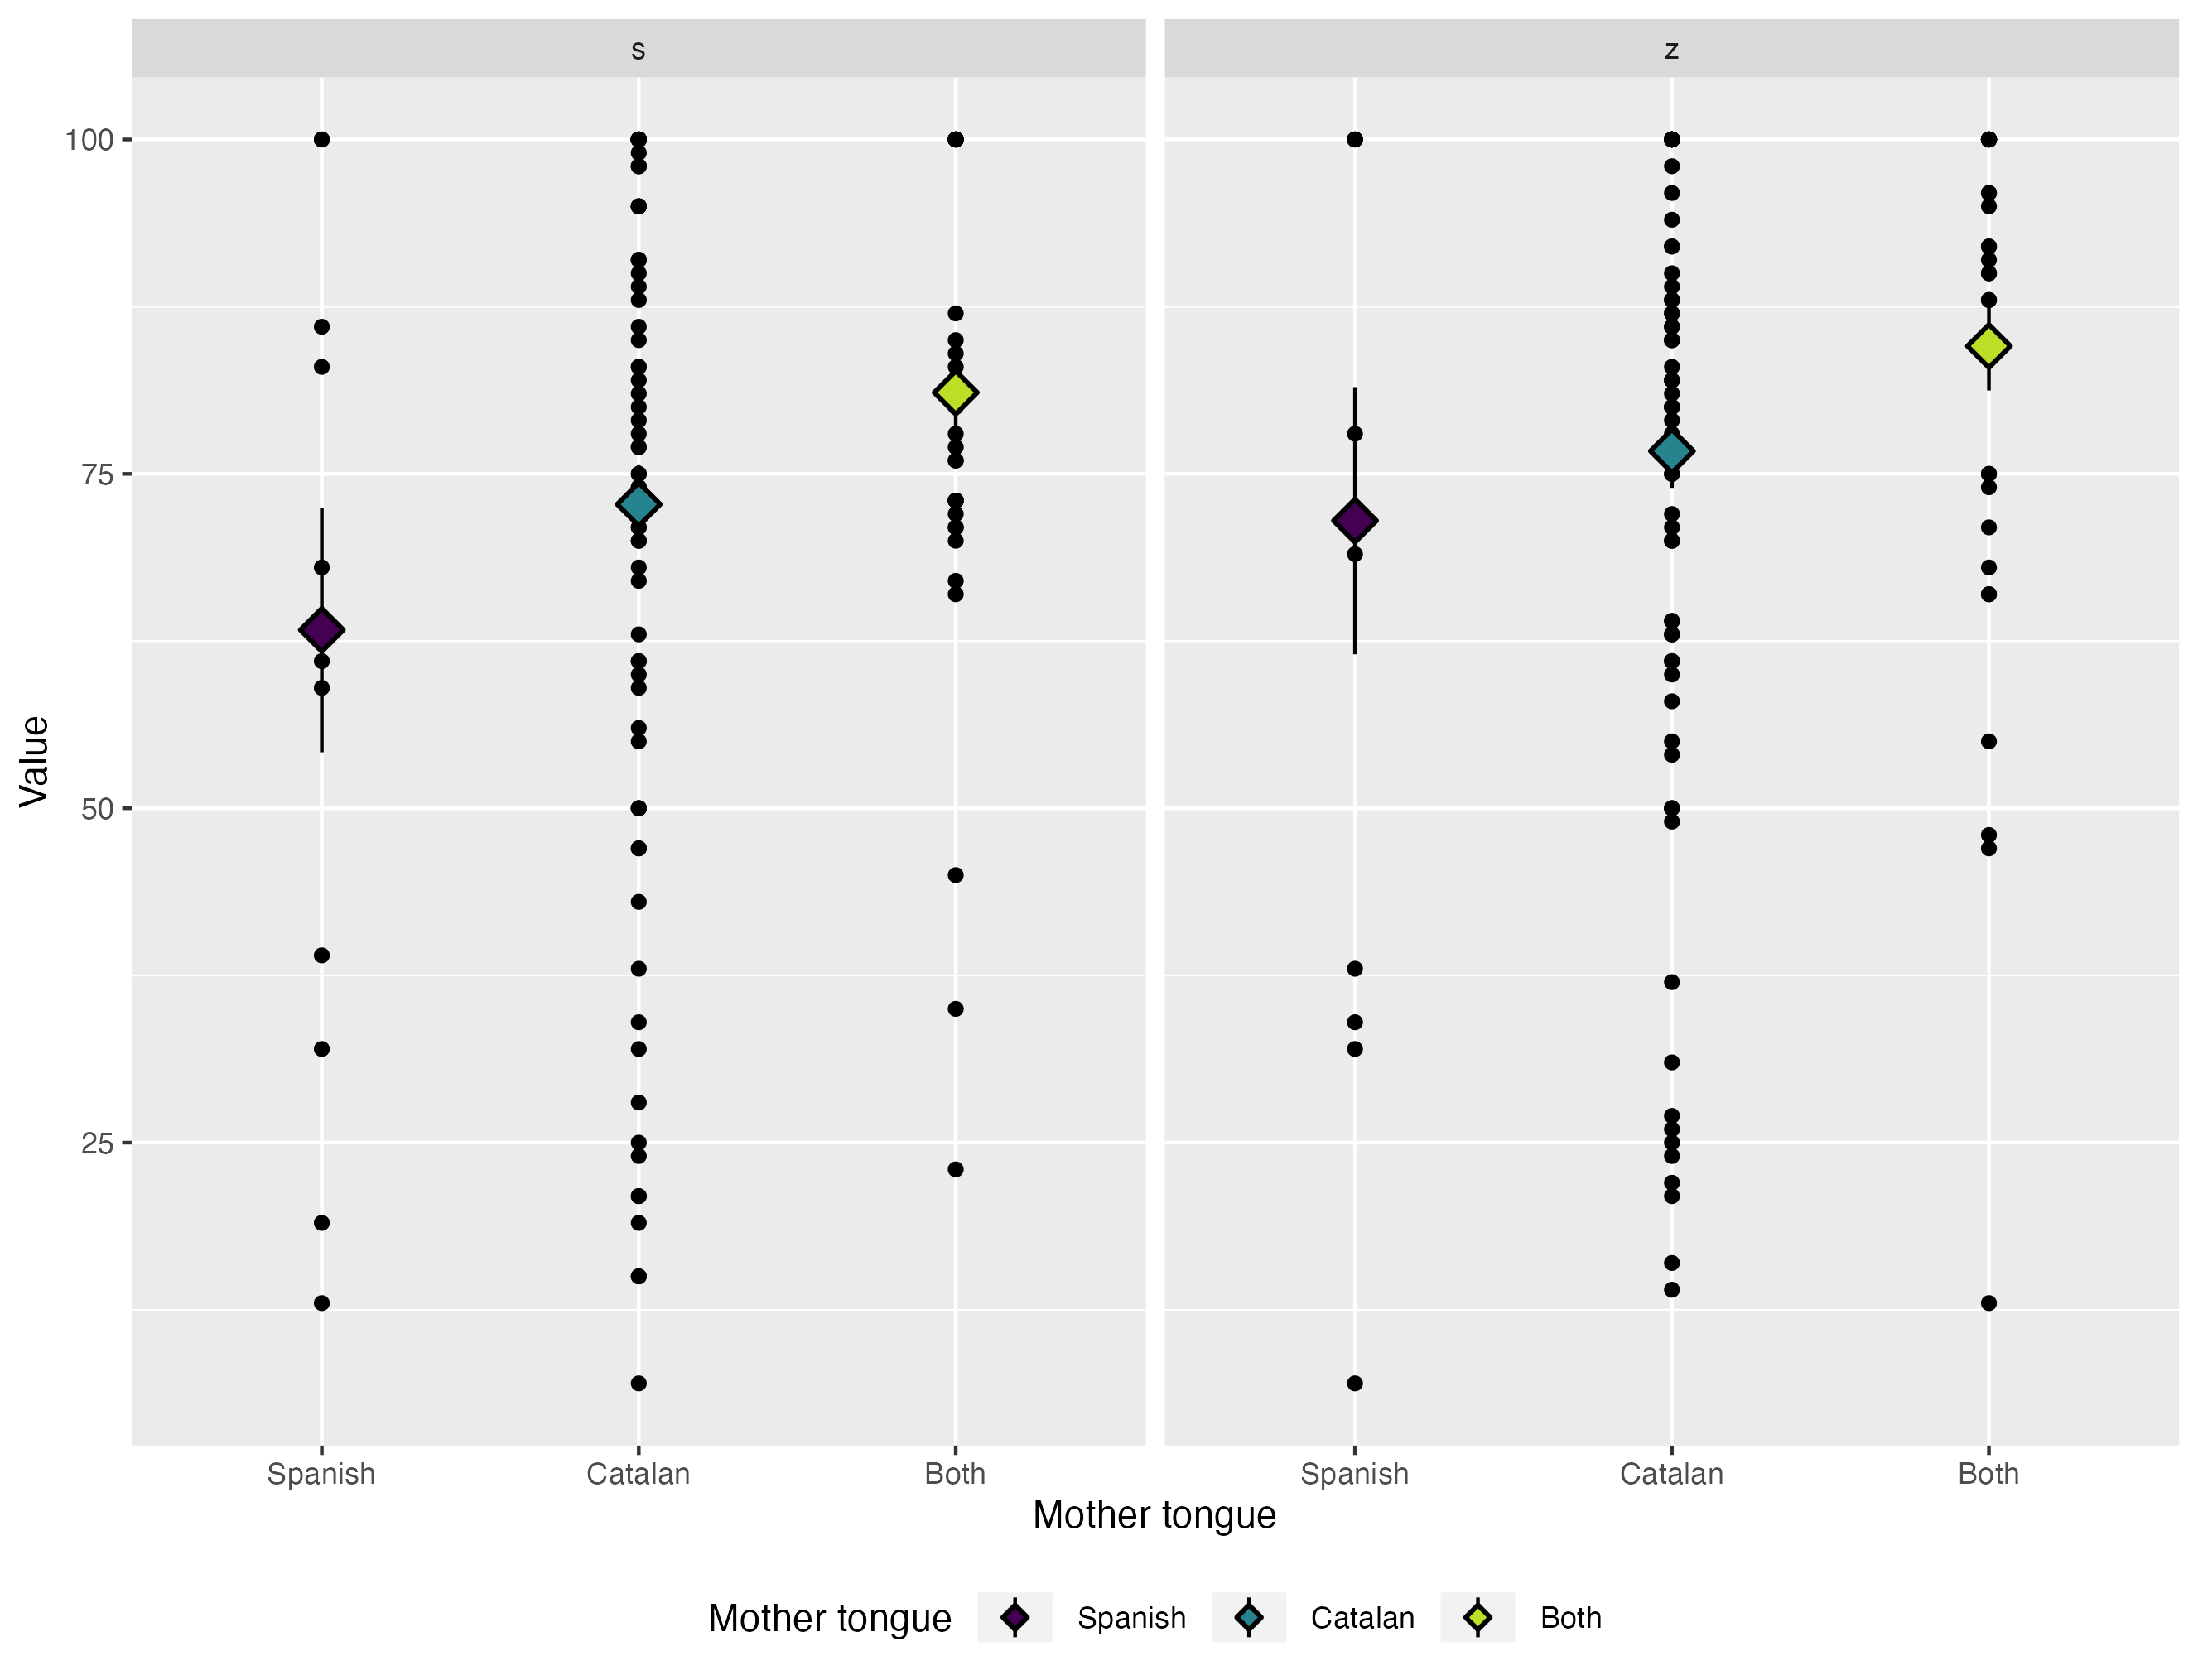
\includegraphics[height=15cm]{./includes/figures/oc.png}
\caption{Ratings of "És d'origen català" as a function of mother tongue}\label{fig:oc}
\end{center}
\end{figure}

Participant responses to the statements \emph{És simpàtic} `S/he is
nice' and \emph{És de fiar} `S/he is trustworthy' showed similar
results, as illustrated in Figures \ref{fig:fiar}. Those who are from
and live in the province of Barcelona give higher ratings to the
speaker, compared to those who are from and live in Girona.

\begin{figure}[!ht]
\begin{center}
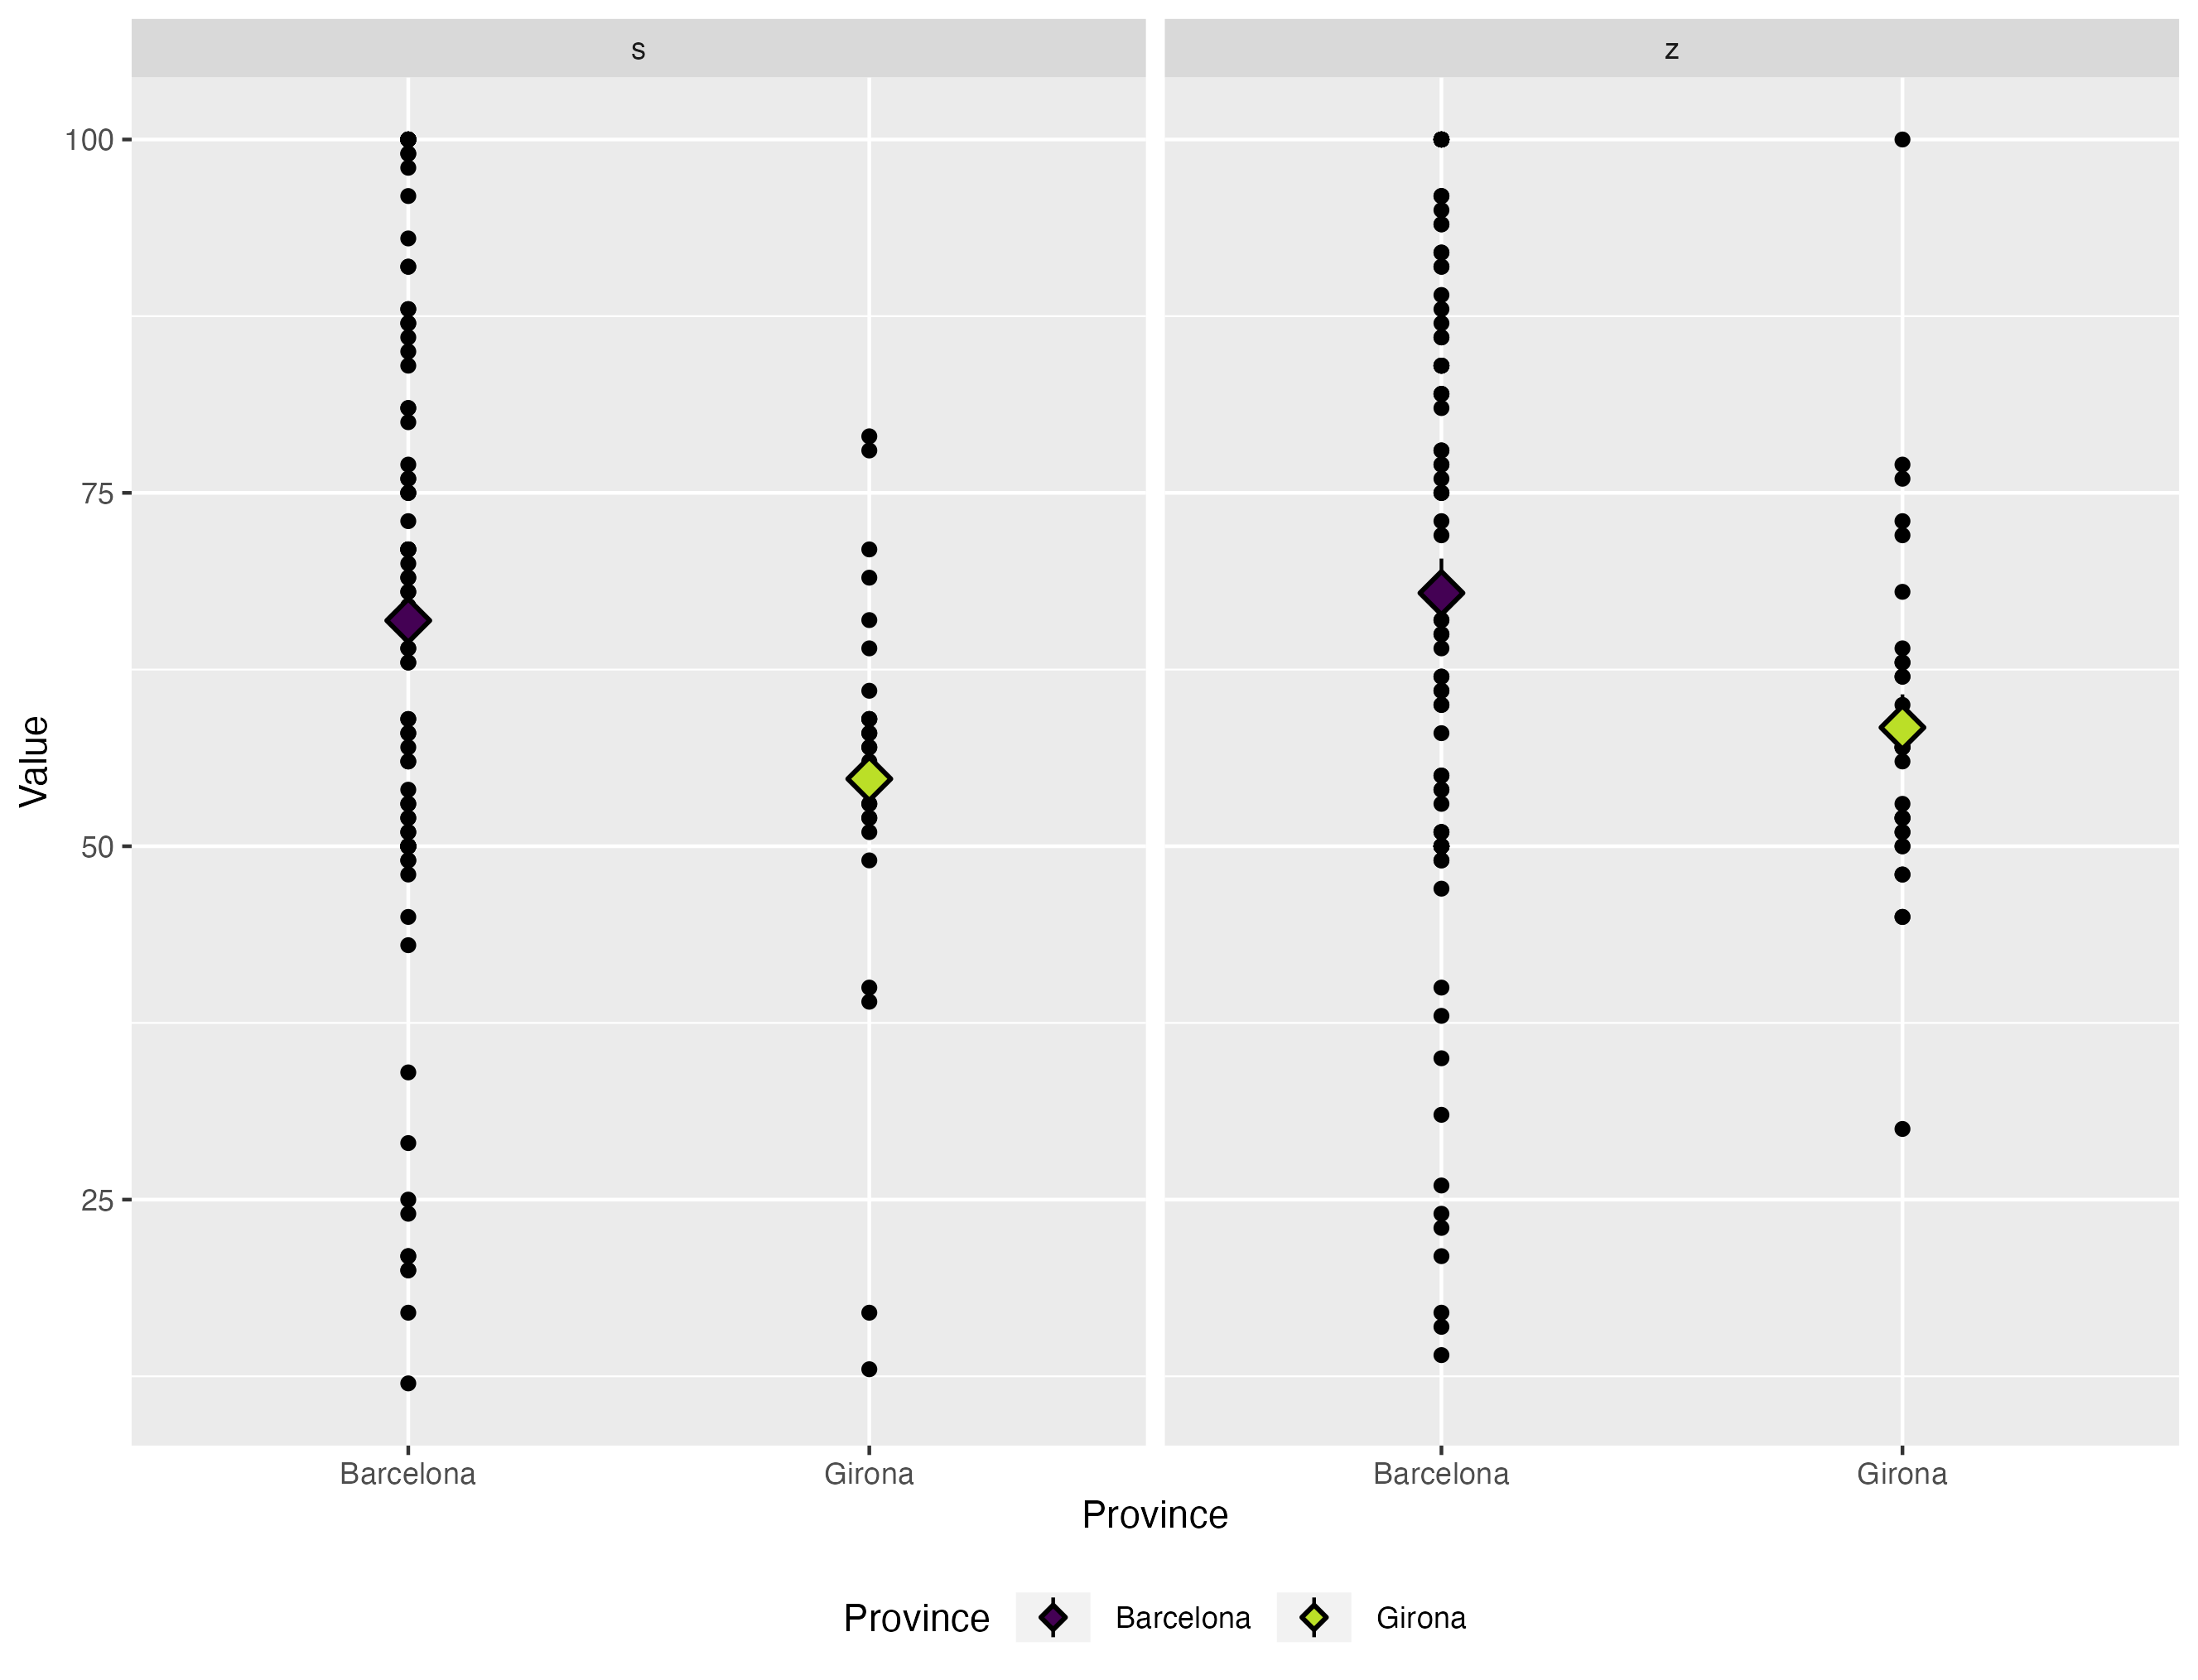
\includegraphics[height=15cm]{./includes/figures/fiar.png}
\caption{Ratings of "És de fiar" as a function of mother tongue}\label{fig:fiar}
\end{center}
\end{figure}

\section{Discussion}

The aim of this exploration study was to explore the covert attitudes
that are linked to the perception Catalan intervocalic /s/ as either
{[}s{]} or {[}z{]} and to examine the relationship between individual
social factors and covert attitudes towards Catalan intervocalic /s/.
The results suggest that these predictors have a different effect on the
ratings of the speaker depending on the social characteristic under
evaluation.

Contrary to what we expected, phoneme was not a significant predictor.
One explanation for this divergent pattern could be that either
participants could not distinguish between {[}s{]} and {[}z{]}
\textbf{(Davidson, 2019)} or, if they could, this difference in
production was not changing their attitudes towards the speaker
\textbf{(Sinner, 2002)}. This finding is interesting considering that
the production of the voiceless alveolar fricative in intervocalic
position has been considered a result of Catalan in contact with Spanish
\textbf{(Benet et al., 2012; Davidson, 2020; Recasens Vives, 1996,
p.~268)}, and, from a prescriptivist point of view, it should be avoided
\textbf{(Institut d'Estudis Catalans, 2022)}. Despite the lack of
significance of this predictor, it should be mentioned that the speaker
received more positive ratings when the {[}z{]} was being produced. The
fact that phoneme was not an important factor contrasts with
\textbf{Davidson (2020)}, who analyzed covert and overt attitudes
towards Catalonian Spanish and found that {[}z{]} was a significant
predictor: it was considered a sociolinguistic indicator of
Catalan-Spanish bilingual membership. Although at this point we can only
hypothesize, it could be that {[}z{]} is perceptually more salient in
Spanish than in Catalan, as the Spanish inventory does not have the
phoneme /z/, but voicing of /s/ might partially occur \textbf{(Benet et
al., 2012; Hualde \& Colina, 2015; Hualde et al., 2020)}. Another
explanation could be that the /s/ alone does not provide enough social
information; rather, the combination of the phoneme /s/ with the
precedent vowel might give the listener more cues and have a stronger
social meaning. Future studies should address this issue in order to
explore if the combination of vowel + /s/ carries other social
connotations than just the /s/ alone.

We expected mother tongue to be a strong predictor of the attitudes
towards the production of intervocalic /s/, specifically, that L1
Catalan and bilingual speakers would give higher rates to those
statements with {[}z{]}. This hypothesis was only partially confirmed.
As reported above, phoneme was not a factor influencing the attitudes,
and mother tongue was only a significant predictor in the two statements
related to Catalan identity, namely \emph{Parla bé català} `S/he speaks
proper Catalan' and \emph{És d'origen català} `S/he is of Catalan
origin'. Interestingly, bilinguals gave higher ratings to the speaker,
followed by L1 Catalan participants and L1 Spanish participants. A
potential explanation for this finding, that should be verified in
future research, could be that L1 Catalan speakers have specific ideas
(higher standards) towards the `proper' Catalan. In addition, some
studies have suggested that those Catalan people who grow up in
Spanish-speaking households typically exhibit more negative attitudes
towards Catalan \textbf{(CITATIONS)}, which is consistent with our
results.

Lastly, province was also found as an important predictor, but only for
some statements. In two of the solidarity statements (\emph{És simpàtic}
`S/he is nice'; \emph{És de fiar} `S/he is trustworthy'), the speaker
was rated more positively by those participants from the province of
Barcelona. This finding might suggest that they identify with the
speaker; thus, giving her higher ratings \textbf{BUSCAR CITA}.
Interestingly, the speaker that created the stimuli is from the province
of Girona, but has spent the last 11 years of her life living outside
that area, either in Barcelona or in another country. We asked her to
read the sentences using a Central Catalan `neutral accent', which
people might have potentially related with Barcelona. This `neutral
accent' does not show any of the prototypical characteristics of the
\emph{accent gironí}, a subvariety within Central Catalan spoken in some
areas of Girona \textbf{(Gros, 2024)}.

\section{Conclusion}

In summary, our findings suggest that the relationship between covert
attitudes and speaker ratings is not straightforward, as the speaker was
evaluated differently based on the social characteristic, with varying
factors influencing such ratings (mother tongue and province).
Crucially, phoneme production did not had an effect on the ratings, even
though prescriptivist norms disfavor the realization of {[}s{]} in
intervocalic position. Future studies should include a larger
participant pool, as well as participants from other regions in
Catalonia, such as Lleida and Tarragona. In addition, examining other
phoneme productions that emerge through the contact of Catalan with
Spanish could give us a better understanding of the factors that affect
the attitudes towards the Catalan language, and potential
sociolinguistic stereotypes and indicators related to Catalan identity.

\bibliographystyle{./includes/bib/IEEEtran.bst}
\bibliography{./includes/bib/icphs2023.bib}

\end{document}
